\section{Mô hình}

% ============================================================
% SLIDE S2
% ============================================================
\SectionSlide{02}{CHƯƠNG 2}{Mô hình D-Tracker}{Trend + Seasonal + Outlier}{%
  \SecItem{2.1}{Big picture: tách thành ba thành phần}
  \SecItem{2.2}{Trend tensor: Tucker + phản ứng--khuếch tán}
  \SecItem{2.3}{Seasonal tensor và outlier tensor}}


% ============================================================
% SLIDE 6
% ============================================================
\begin{frame}{Big picture: tách cửa sổ thành ba thành phần}{Tổng quan}
\begin{columns}[c,onlytextwidth]
\begin{column}{0.58\textwidth}
\centering
\begin{tikzpicture}[x=.72cm,y=.5cm]
  % observed = trend + season + outlier
  \node[tinylabel,anchor=west] at (0,8.6) {\textbf{Quan sát} $\mathcal X_c$ (một chuỗi, minh họa)};
  \draw[DTNavy,line width=1.1pt] plot[domain=0:7,samples=90]
    (\x,{6.1+.25*\x+.45*sin(155*\x)}) ;
  \draw[DTNavy,line width=1.1pt] (4.6,{6.1+.25*4.6+.45*sin(155*4.6)}) -- (4.7,8.0) -- (4.8,{6.1+.25*4.8+.45*sin(155*4.8)});
  \node at (3.5,5.0) {\Large$\approx$};
  \node[tinylabel,text=DTTeal,anchor=west] at (0,4.25) {\textbf{Trend} $\widehat{\mathcal X}_d$};
  \draw[DTTeal,line width=1.1pt] plot[domain=0:7,samples=40] (\x,{2.9+.25*\x});
  \node[font=\small] at (7.6,3.7) {$+$};
  \node[tinylabel,text=DTGold,anchor=west] at (0,2.05) {\textbf{Seasonal} $\widehat{\mathcal X}_s$};
  \draw[DTGold,line width=1.1pt] plot[domain=0:7,samples=90] (\x,{1.2+.45*sin(155*\x)});
  \node[font=\small] at (7.6,1.2) {$+$};
  \node[tinylabel,text=DTClaret,anchor=west] at (0,-.05) {\textbf{Outlier} $\widehat{\mathcal X}_o$};
  \draw[DTClaret] (0,-.9) -- (7,-.9);
  \draw[DTClaret,line width=1.3pt] (4.7,-.9) -- (4.7,.2);
  \fill[DTClaret] (4.7,.2) circle (.1);
\end{tikzpicture}
\end{column}
\begin{column}{0.40\textwidth}
  \small Thách thức chính: \textbf{trend và lan truyền bị che} bởi mùa vụ và ngoại lai.\par
  \vspace{2mm}
  \formula{\mathcal X_c \;\approx\; \widehat{\mathcal X}_d+\widehat{\mathcal X}_s+\widehat{\mathcal X}_o}
  \vspace{1mm}
  {\scriptsize\color{DTMuted}cả ba cùng kích thước $k\times l\times L_c$\par}
  \vspace{2mm}
  \begin{itemize}\small
    \item {\color{DTTeal}\textbf{Trend tensor}}: xu hướng + \textbf{lan truyền}.
    \item {\color{DTGold}\textbf{Seasonal tensor}}: mẫu lặp theo chu kỳ.
    \item {\color{DTClaret}\textbf{Outlier tensor}}: điểm bất thường, \textbf{rất thưa}.
  \end{itemize}
\end{column}
\end{columns}
\vfill
\papersource{§3.3, Eq.~(1), Figure 2.}
\end{frame}

% ============================================================
% SLIDE 7
% ============================================================
\begin{frame}{Trend tensor: vì sao phải gom nhóm?}{Trend tensor}
\begin{columns}[c,onlytextwidth]
\begin{column}{0.52\textwidth}
\centering
\begin{tikzpicture}[x=1cm,y=1cm]
  \foreach \i in {0,...,22}{
    \pgfmathsetmacro{\a}{0.15+0.04*mod(\i*7,11)}
    \pgfmathsetmacro{\b}{0.3+0.11*mod(\i*5,13)}
    \draw[DTMuted!45,line width=.35pt] plot[domain=0:2.6,samples=14] (\x,{\b+\a*\x+.12*sin(240*\x+40*\i)});
  }
  \node[tinylabel,align=center] at (1.3,-0.45) {$k\cdot l = 8\times 50 = 400$ chuỗi};
  \draw[dtarrow] (2.85,1.2) -- (3.75,1.2);
  \node[tinylabel] at (3.3,1.55) {gom};
  \draw[DTTeal,line width=1.2pt] plot[domain=4:6.6,samples=20] (\x,{0.4+0.25*(\x-4)});
  \draw[DTBlue,line width=1.2pt] plot[domain=4:6.6,samples=20] (\x,{1.0+0.06*(\x-4)^2});
  \draw[DTGold,line width=1.2pt] plot[domain=4:6.6,samples=20] (\x,{2.0-0.2*(\x-4)});
  \draw[DTClaret,line width=1.2pt] plot[domain=4:6.6,samples=20] (\x,{1.6+0.12*(\x-4)});
  \draw[DTNavy,line width=1.2pt] plot[domain=4:6.6,samples=20] (\x,{0.15+0.02*(\x-4)});
  \draw[DTTeal!60!DTGold,line width=1.2pt] plot[domain=4:6.6,samples=20] (\x,{2.5-0.05*(\x-4)});
  \node[tinylabel,align=center] at (5.3,-0.45) {$d_k\cdot d_l = 3\times 2 = 6$ chuỗi ẩn};
\end{tikzpicture}
\end{column}
\begin{column}{0.45\textwidth}
  \small
  \textbf{Mô hình từng cặp (keyword, location)}:
  quá nhiều tham số $\Rightarrow$ overfit, chậm, khó đọc.\par
  \vspace{2mm}
  \textbf{Ý tưởng}: gom
  \begin{itemize}
    \item từ khóa $\rightarrow$ $d_k$ \textbf{nhóm chủ đề ẩn},
    \item địa điểm $\rightarrow$ $d_l$ \textbf{nhóm vùng ẩn},
  \end{itemize}
  với $d_k\ll k$, $d_l\ll l$.
  \vspace{2mm}
  \begin{intuition}[``Yếu tố ẩn'' là gì?]
    Một \textbf{nhóm mềm}: mỗi từ khóa / nước thuộc về mỗi nhóm với một \textbf{mức độ} $\ge 0$, không phải 0/1.
  \end{intuition}
  \vspace{1mm}
  Lợi ích: tín hiệu mạnh hơn (gộp nhiễu), dễ diễn giải, tính nhanh hơn.
\end{column}
\end{columns}
\vfill
\papersource{§3.3; ví dụ $d_k=3$, $d_l=2$ lấy từ Figure 1(b).}
\end{frame}

% ============================================================
% SLIDE 8
% ============================================================
\begin{frame}{Phân rã Tucker: $\mathcal W^{(\mathrm{core})}$, $W^{(\mathrm{key})}$, $W^{(\mathrm{loc})}$}{Trend tensor}
\formula{\widehat{\mathcal X}_d \;=\; \mathcal W^{(\mathrm{core})} \times_{\mathrm{key}} W^{(\mathrm{key})} \times_{\mathrm{loc}} W^{(\mathrm{loc})}}
\vspace{2mm}
\begin{columns}[T,onlytextwidth]
\begin{column}{0.50\textwidth}
\begin{questioncard}
\small
\begin{tabular}{@{}l@{\;}l@{}}
  $\mathcal W^{(\mathrm{core})}\in\mathbb R^{d_k\times d_l\times L_c}$ & \textbf{động thái ẩn} \\[1mm]
  $W^{(\mathrm{key})}\in\mathbb R_+^{d_k\times k}$ & từ khóa $\to$ nhóm \\[1mm]
  $W^{(\mathrm{loc})}\in\mathbb R_+^{d_l\times l}$ & nước $\to$ nhóm vùng
\end{tabular}
\end{questioncard}

\vspace{3mm}
\textbf{Mode product nói bằng lời:}
$\times_{\mathrm{key}}$ trộn các nhóm từ khóa thành từ khóa thật,
$\times_{\mathrm{loc}}$ trộn các nhóm vùng thành nước thật.
\end{column}
\begin{column}{0.47\textwidth}
\begin{intuition}[Một phần tử]
  \centering
  $\displaystyle \hat x_{uv}(t)=\sum_{i=1}^{d_k}\sum_{j=1}^{d_l}
  W^{(\mathrm{key})}_{iu}\,W^{(\mathrm{loc})}_{jv}\,w_{ij}(t)$\par
  \vspace{1mm}
  \raggedright\small Chuỗi ``iPhone tại Việt Nam'' = \textbf{tổng có trọng số} của các chuỗi ẩn.
\end{intuition}
\vspace{2mm}
\begin{takeaway}[Vì sao không âm?]
  \small Trọng số $\ge 0$ thì không ``đảo dấu'' câu chuyện $\Rightarrow$ câu chuyện ở không gian ẩn vẫn đúng khi chiếu về dữ liệu thật.
\end{takeaway}
\end{column}
\end{columns}
\vfill
\papersource{§3.3, Eq.~(2). Định nghĩa mode product: Appendix A1.}
\end{frame}

% ============================================================
% SLIDE 9
% ============================================================
\begin{frame}{Động thái ẩn sinh ra từ hệ phản ứng--khuếch tán}{Reaction--diffusion}
\begin{columns}[T,onlytextwidth]
\begin{column}{0.55\textwidth}
  {\small Gốc hóa học: chất đi từ nơi \textbf{nồng độ cao} sang nơi \textbf{nồng độ thấp}.\par}
  \vspace{1mm}
  \begin{mathcard}[D-Tracker áp lên $\mathcal W^{(\mathrm{core})}$ (Eq.~3)]
  \centering
  $\displaystyle \frac{dw_{ij}}{dt}=
  \underbrace{\colorbox{DTTeal!12}{$a_{ij}\,w_{ij}$}}_{\text{phản ứng}}
  +\underbrace{\colorbox{DTGold!18}{$\sum_{j'} d_{ijj'}\,(w_{ij'}-w_{ij})$}}_{\text{khuếch tán}}$
  \end{mathcard}
  \vspace{1mm}
  \small
  \begin{itemize}
    \item $w_{ij}(t)$: mức quan tâm của \textbf{nhóm từ khóa} $i$ tại \textbf{nhóm vùng} $j$.
    \item {\color{DTTeal}$a_{ij}$}: tốc độ tăng tự thân; $>0$ tăng, $<0$ giảm.
    \item {\color{DTGold!80!black}$d_{ijj'}\ge 0$}: cường độ lan của nhóm $i$ \textbf{từ vùng $j'$ sang vùng $j$}.
      Nếu $w_{ij'}>w_{ij}$ thì $w_{ij}$ bị kéo lên.
  \end{itemize}
\end{column}
\begin{column}{0.42\textwidth}
\centering
\begin{tikzpicture}[x=.85cm,y=.72cm]
  % two tanks
  \draw[DTNavy,line width=.8pt] (0,0) rectangle (1.6,2.4);
  \fill[DTTeal!45] (0,0) rectangle (1.6,1.9);
  \draw[DTNavy,line width=.8pt] (3.2,0) rectangle (4.8,2.4);
  \fill[DTTeal!45] (3.2,0) rectangle (4.8,0.7);
  \draw[DTNavy,line width=.8pt] (1.6,0.25) -- (3.2,0.25);
  \draw[DTNavy,line width=.8pt] (1.6,0.45) -- (3.2,0.45);
  \draw[-{Latex[length=2mm]},DTGold,line width=1.4pt] (1.8,0.35) -- (3.0,0.35);
  \node[font=\scriptsize,text=DTGold!80!black] at (2.4,0.75) {$d_{ijj'}$};
  \node[font=\small\bfseries,text=DTNavy] at (0.8,-0.35) {vùng $j'$};
  \node[font=\small\bfseries,text=DTNavy] at (4.0,-0.35) {vùng $j$};
  \node[font=\scriptsize,text=DTMuted] at (0.8,1.6) {$w_{ij'}$ cao};
  \node[font=\scriptsize,text=DTMuted] at (4.0,1.0) {$w_{ij}$ thấp};
  % taps
  \draw[-{Latex[length=2mm]},DTTeal,line width=1.2pt] (0.8,3.1) -- (0.8,2.5);
  \draw[-{Latex[length=2mm]},DTTeal,line width=1.2pt] (4.0,3.1) -- (4.0,2.5);
  \node[font=\scriptsize,text=DTTeal] at (0.8,3.35) {$a_{ij'}$};
  \node[font=\scriptsize,text=DTTeal] at (4.0,3.35) {$a_{ij}$};
\end{tikzpicture}

\vspace{1mm}
\begin{intuition}[Quy mô]
  \small $d_k d_l$ phương trình; $A\in\mathbb R^{d_k\times d_l}$, $\mathcal D\in\mathbb R_+^{d_k\times d_l\times d_l}$.
  Chỉ lan \textbf{giữa các nhóm vùng}, trong cùng nhóm từ khóa.
\end{intuition}
\end{column}
\end{columns}
\vfill
\papersource{§3.2, §3.3, Eq.~(3).}
\end{frame}

% ============================================================
% SLIDE 10
% ============================================================
\begin{frame}{Trực giác: phản ứng và khuếch tán ngoài đời}{Reaction--diffusion}
\begin{columns}[T,onlytextwidth]
\begin{column}{0.53\textwidth}
\small
\renewcommand{\arraystretch}{1.15}
\begin{tabular}{@{}>{\raggedright\arraybackslash}p{1.45cm}>{\raggedright\arraybackslash}p{2.7cm}>{\raggedright\arraybackslash}p{2.7cm}@{}}
  \toprule
  & \textbf{COVID-19} & \textbf{iPhone mới} \\
  \midrule
  {\color{DTTeal}\textbf{Phản ứng}} $a_{ij}$
  & Tốc độ lây \emph{trong} một thành phố, tùy chính sách giãn cách.
  & Sức hút tự thân tại một thị trường (quảng cáo, truyền thông). \\[1mm]
  {\color{DTGold!80!black}\textbf{Khuếch tán}} $d_{ijj'}$
  & Người dân đi lại giữa các thành phố $\Rightarrow$ dịch lan từ vùng nặng sang vùng nhẹ.
  & Quan tâm lan qua biên giới, từ thị trường ``nóng'' sang thị trường khác. \\
  \bottomrule
\end{tabular}
\vspace{2mm}
\begin{caution}[Giả định của paper]
  Quan tâm lan từ nơi \textbf{cao} sang nơi \textbf{thấp}, giống chất hóa học. Ví dụ COVID là minh họa của nhóm.
\end{caution}
\end{column}
\begin{column}{0.44\textwidth}
  \centering
  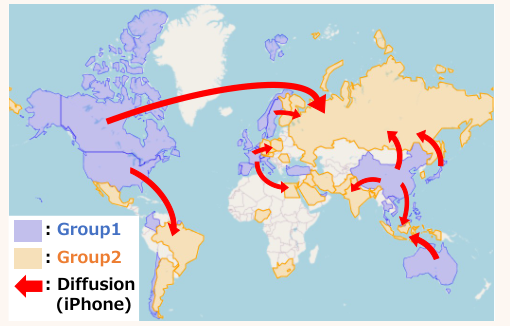
\includegraphics[width=\linewidth]{figures/Figure1b_diffusion_2019.png}\par
  \vspace{1mm}
  {\scriptsize\color{DTMuted}Kết quả thật (Device, 04/2019--03/2021): quan tâm ``iPhone'' lan từ Mỹ, châu Âu, Trung Quốc (Group 1) sang phần còn lại (Group 2).}
\end{column}
\end{columns}
\vfill
\papersource{§3.2; §1.1, Figure 1(b).}
\end{frame}

% ============================================================
% SLIDE 11
% ============================================================
\begin{frame}{Từ phương trình đến $\mathcal W^{(\mathrm{core})}$ và dự báo}{Trend tensor}
\centering
\begin{tikzpicture}[x=1cm,y=.5cm]
  \draw[->,DTMuted] (0,0) -- (13.2,0) node[right,font=\scriptsize] {$t$};
  \draw[DTTeal,line width=1.3pt] plot[domain=0:8,samples=40] (\x,{0.4+0.9*(1-exp(-0.25*\x))+0.012*\x*\x});
  \draw[DTTeal,line width=1.3pt,dashed] plot[domain=8:12.5,samples=30] (\x,{0.4+0.9*(1-exp(-0.25*\x))+0.012*\x*\x});
  \draw[DTGold,line width=1.3pt] plot[domain=0:8,samples=40] (\x,{1.8-0.08*\x});
  \draw[DTGold,line width=1.3pt,dashed] plot[domain=8:12.5,samples=30] (\x,{1.8-0.08*\x});
  \fill[DTNavy] (0,0.4) circle (.07) node[left,font=\scriptsize] {$w_0$};
  \fill[DTNavy] (0,1.8) circle (.07);
  \draw[DTMuted,dashed] (8,0) -- (8,4.6);
  \node[font=\scriptsize,text=DTMuted,below] at (8,0) {$t_c$};
  \draw[decorate,decoration={brace,amplitude=5pt},DTNavy] (0,4.7) -- (8,4.7)
    node[midway,above=5pt,font=\small,text=DTNavy] {giải số $L_c$ bước $\Rightarrow$ \textbf{khớp} cửa sổ hiện tại};
  \draw[decorate,decoration={brace,amplitude=5pt},DTGold] (8,4.7) -- (12.5,4.7)
    node[midway,above=5pt,font=\small,text=DTGold!80!black] {chạy tiếp $L_f$ bước $\Rightarrow$ \textbf{dự báo}};
\end{tikzpicture}

\vspace{2mm}
\begin{columns}[T,onlytextwidth]
\begin{column}{0.49\textwidth}
\begin{mathcard}[Definition 1 --- hệ phản ứng--khuếch tán]
  \small $\theta=\{A,\mathcal D\}$.\\
  $f_\theta(\theta,w_0,L)$: sinh chuỗi $\mathcal W^{(\mathrm{core})}$ dài $L$ từ $w_0$.\\
  {\scriptsize\color{DTMuted}Device: $A$ có 6 số, $\mathcal D$ có 12 số.}
\end{mathcard}
\end{column}
\begin{column}{0.49\textwidth}
\begin{mathcard}[Definition 2 --- trend tensor]
  \small $\theta_d=\{W^{(\mathrm{key})},W^{(\mathrm{loc})},\theta\}$.\\
  Dự báo trend = chiếu $\mathcal W^{(\mathrm{core})}$ tương lai qua $W^{(\mathrm{key})}, W^{(\mathrm{loc})}$.
\end{mathcard}
\end{column}
\end{columns}
\vfill
\papersource{Def.~1--2. Chiếu đạo hàm về từng chuỗi thật: Appendix A2.}
\end{frame}

% ============================================================
% SLIDE 12
% ============================================================
\begin{frame}{Seasonal tensor: nén mùa vụ vào ba ma trận}{Seasonal tensor}
\formula{\widehat{\mathcal X}_s = S^{(\mathrm{time})}\times_{\mathrm{key}} S^{(\mathrm{key})}\times_{\mathrm{loc}} S^{(\mathrm{loc})}
\qquad
\hat x^{s}_{uv}(t)=\sum_{r=1}^{d_s} S^{(\mathrm{key})}_{ru}\,S^{(\mathrm{loc})}_{rv}\,S^{(\mathrm{time})}_{rt}}
\vspace{2mm}
\begin{columns}[T,onlytextwidth]
\begin{column}{0.32\textwidth}
\begin{questioncard}
  \textbf{$S^{(\mathrm{time})}\in\mathbb R^{d_s\times L_c}$}\par
  \small $d_s$ \textbf{đường cong chu kỳ chuẩn}, mỗi cột là một bước thời gian.\par
  \vspace{1mm}
  \scriptsize\color{DTMuted} vd: ``đỉnh mùa thu'' (ra máy), ``đỉnh cuối năm'' (Black Friday).
\end{questioncard}
\end{column}
\begin{column}{0.32\textwidth}
\begin{questioncard}
  \textbf{$S^{(\mathrm{key})}\in\mathbb R^{d_s\times k}$}\par
  \small Từ khóa nào \textbf{ăn khớp} với mẫu chu kỳ nào.\par
  \vspace{2mm}
  \scriptsize\color{DTMuted} vd: iPhone, Apple Watch nặng ở mẫu ``mùa thu''; Galaxy nhẹ hơn.
\end{questioncard}
\end{column}
\begin{column}{0.32\textwidth}
\begin{questioncard}
  \textbf{$S^{(\mathrm{loc})}\in\mathbb R^{d_s\times l}$}\par
  \small Mẫu đó \textbf{mạnh / yếu} ở nước nào.\par
  \vspace{2mm}
  \scriptsize\color{DTMuted} vd: ``Black Friday'' mạnh ở Mỹ, yếu ở Việt Nam; mẫu ``Tết'' chỉ ở châu Á.
\end{questioncard}
\end{column}
\end{columns}
\vspace{2mm}
\begin{mathcard}[Definition 3]
  \small $\theta_s=\{S^{(\mathrm{time})},S^{(\mathrm{key})},S^{(\mathrm{loc})}\}$: thay vì lưu $k\,l\,L_c$ số, chỉ lưu $d_s(L_c+k+l)$ số.
\end{mathcard}
\vfill
\papersource{Eq.~(4), Def.~3. Ví dụ Black Friday/Tết là minh họa của nhóm.}
\end{frame}

% ============================================================
% SLIDE 13
% ============================================================
\begin{frame}{Outlier tensor và bộ tham số đầy đủ}{Outlier \& regime}
\begin{columns}[T,onlytextwidth]
\begin{column}{0.40\textwidth}
  \begin{itemize}\small
    \item $\widehat{\mathcal X}_o$ chỉ chứa \textbf{giá trị bất thường}. Giả định chúng hiếm $\Rightarrow$ tensor \textbf{thưa} (gần như toàn 0).
  \end{itemize}
  \vspace{1mm}
  \begin{mathcard}[Definition 4 --- một mô hình]
    \small $\Theta=\{\theta_d,\theta_s,\widehat{\mathcal X}_o\}$\\
    mô tả trend, lan truyền, mùa vụ, ngoại lai của \textbf{một giai đoạn}.
  \end{mathcard}
  \vspace{1.5mm}
  \begin{mathcard}[Definition 5 --- toàn bộ D-Tracker]
    \small $\mathcal F=\{\Theta_1,\Theta_2,\dots,\Theta_N\}$\\
    $N$ mô hình cho $N$ \textbf{giai đoạn (regime)}. Khi hành vi đổi, D-Tracker \textbf{đổi mô hình}.
  \end{mathcard}
\end{column}
\begin{column}{0.57\textwidth}
  \centering
  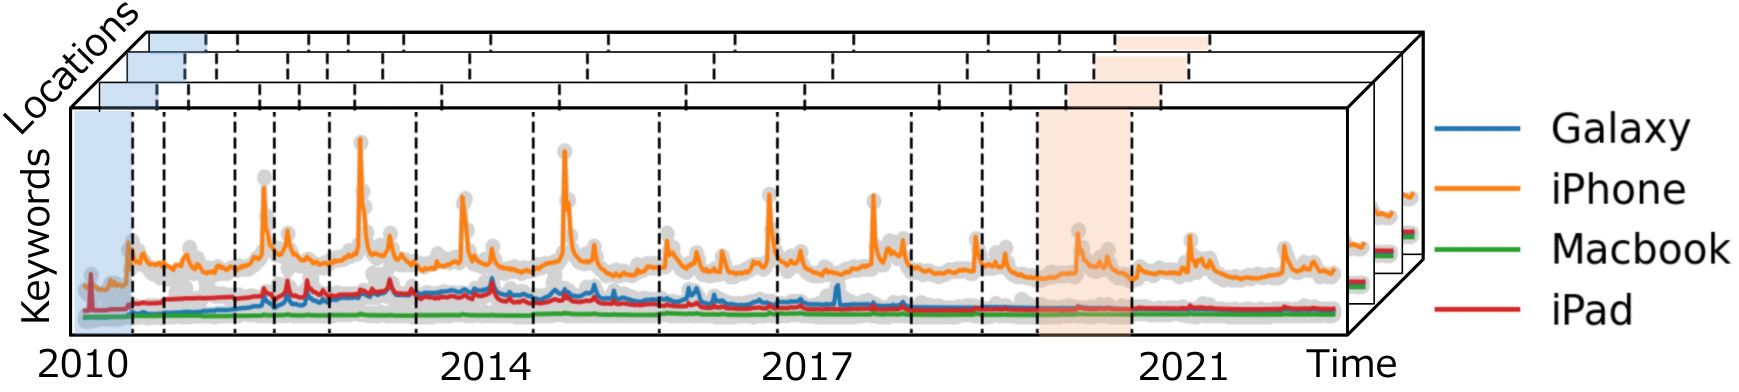
\includegraphics[width=\linewidth]{figures/Figure1_a.png}\par
  \vspace{1mm}
  {\scriptsize\color{DTMuted}Đường chấm dọc = thời điểm D-Tracker tự động đổi sang mô hình mới.
  Mỗi đoạn giữa hai đường chấm dùng một $\Theta$.}
  \vspace{3mm}
  \begin{caution}[Đừng nhầm]
    \small $\mathcal F$ \textbf{không} phải mỗi observation một $\Theta$, mà là mỗi \textbf{giai đoạn} một $\Theta$.
  \end{caution}
\end{column}
\end{columns}
\vfill
\papersource{Def.~4--5, Figure 1(a).}
\end{frame}
